\documentclass{article}% For the example only, any class will do

\usepackage{amsmath}
\usepackage{booktabs}
\usepackage{float}
\usepackage{graphicx}
\usepackage{pgf, tikz}
\usepackage{multicol}
\usepackage[left=0.01cm,right=0.01cm,top=0cm,bottom=0cm,paperwidth=8.3cm,paperheight=12.5cm]{geometry}
\usepackage{enumitem}
\usetikzlibrary{positioning}
\usetikzlibrary{arrows}
\setlength\parindent{0pt}
% \newcommand{\specialcell}[2][c]{%
%   \begin{tabular}[#1]{@{}c@{}}#2\end{tabular}}

\begin{document}

	% \begin{tikzpicture}[->,node distance=2cm,ultra thick]
%
% 		\node (pij) [rectangle,rounded corners,dashed,draw=red] {$p_{ij}$};
% 		\node (Nij) [rectangle,rounded corners,draw=black,below of=pij] {$N_{ij}$};
% 		\draw [->] (pij) edge (Nij);
% 		\node (Ni) [rectangle,rounded corners,draw=black,left of=Nij] {$N_i$};
% 		\draw [->] (Ni) edge (Nij);
% 		\node (paramN) [circle,draw=black,left of=Ni] {$(\mu_N, \sigma^2_N$)};
% 		\draw [->] (paramN) edge (Ni);
% 		\node (paramp) [circle,draw=black,above of=pij] {$(\pi_j, \mu_j, \sigma^2_j)$};
% 		\draw [->] (paramp) edge (pij);
% 		\node (F) [circle,draw=black,above of=paramp] {$F$};
% 		\draw [->] (F) edge (paramp);
% 	\end{tikzpicture}

	% \begin{tikzpicture}[->,node distance=1cm,ultra thick]
% 		% array of ps
% 		\node (p1d) {$p_{1d}$};
% 		\node (p2d) [right of = p1d] {$\dots$};
% 		\node (pnd) [right of = p2d] {$p_{nd}$};
% 		\node (p12) [above of = p1d] {$\ \ \vdots\ \ $};
% 		\node (p11) [above of = p12] {$p_{11}$};
% 		\node (p21) [right of = p11] {$\dots$};
% 		\node (pn1) [right of = p21] {$p_{n1}$};
% 		\node (p22) [right of = p12] {$\vdots$};
% 		\node (pn2) [above of = pnd] {$\vdots$};
% 		% the per-feature parameters
% 		\node (param1) [left =0.5cm of p11] {$(\pi_1, \mu_1, \sigma^2_1)$};
% 		\draw [->] (param1) edge (p11);
% 		\node (paramd) [left =0.5cm of p1d] {$(\pi_d, \mu_d, \sigma^2_d)$};
% 		\draw [->] (paramd) edge (p1d);
% 		\node (param2) [below of = param1] {$\ \ \ \vdots\ \ \ \ $};
% 		\draw [->] (param2) edge (p12);
% 		% hpyer parameter
% 		\node (F) [left =1cm of param2] {$F$};
% 		\draw [->] (F) edge (param1);
% 		\draw [->] (F) edge (param2);
% 		\draw [->] (F) edge (paramd);
%
% 		% times
% 		\node (times) [below of = p2d] {$\times$};
%
% 		% array of Ns
% 		\node (N2) [below of = times] {$\dots$};
% 		\node (N1) [left of = N2] {$N_1$};
% 		\node (Nd) [right of = N2] {$N_d$};
% 		%N parameter
% 		\node (paramN) [left =0.5cm of N1] {$(\mu_N, \sigma^2_N)$};
% 				\draw [->] (paramN) edge (N1);
%
% 		% equals
% 		\node (equals) [below of = N2] {\rotatebox{90}{$\,=$}};
%
% 		% array of Nijs
% 		% array of ps
% 		\node (N21) [below of = equals] {$\dots$};
% 		\node (N11) [left of = N21] {$N_{11}$};
% 		\node (NN1) [right of = N21] {$N_{N1}$};
% 		\node (N12) [below of = N11] {$\vdots$};
% 		\node (N22) [below of = N21] {$\vdots$};
% 		\node (NN2) [below of = NN1] {$\vdots$};
% 		\node (N1d) [below of = N12] {$N_{1d}$};
% 		\node (N2d) [below of = N22] {$\dots$};
% 		\node (NNd) [below of = NN2] {$N_{Nd}$};
%
% 	\end{tikzpicture}

\begin{center}

	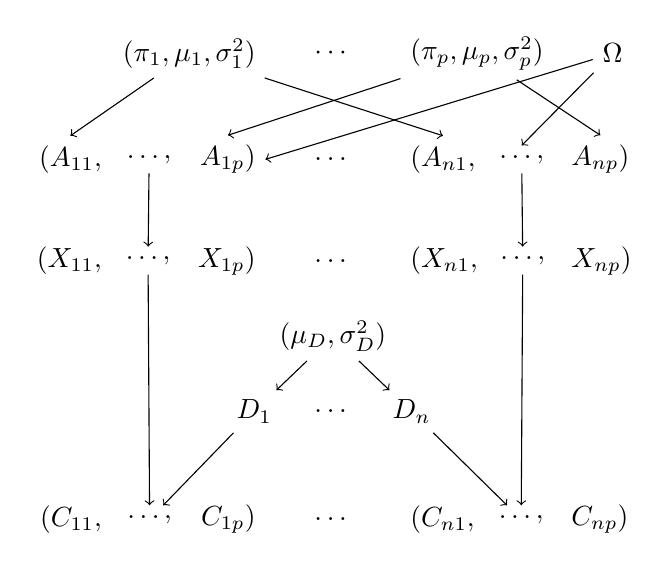
\begin{tikzpicture}[->,node distance=1cm]

%		% F
%		\node (F) {$F$};
		
		% per-feature parameters
%		\node (theta2) [below of = F] {$\cdots$};
		\node (theta2) {$\cdots$};
		\node (theta1) [left = 0.5cm of theta2] {$(\pi_1, \mu_1, \sigma^2_1)$};
		\node (thetam) [right = 0.5cm of theta2] {$(\pi_p, \mu_p, \sigma^2_p)$};
		\node (Omega) [right = 0.5cm of thetam] {$\Omega$};
		
%		\draw [->] (F) edge (theta1);
		% \draw [->] (F) edge (theta2);
%		\draw [->] (F) edge (thetam);
		
		% array of As
		\node (A2) [below = 1cm of theta2] {$\dots$};
%		\node (N1_holder) [left of = A2] {};
		\node (A1p) [left = 0.5cm of A2] {$A_{1p})$};
		\node (A12) [left of = A1p] {$\dots,$};
		\node (A11) [left of = A12] {$(A_{11},$};
		\node (An1) [right = 0.5cm of A2] {$(A_{n1},$};
		\node (An2) [right of = An1] {$\dots,$};
		\node (Anp) [right of = An2] {$A_{np})$};
		
		
		\path [->] (theta1) edge (A11.north);
		% \draw [->] (theta1) edge (p2);
		\draw [->] (theta1) edge (An1.north);
		\draw [->] (thetam) edge (A1p.north);
		% \draw [->] (thetam) edge (p2);
		\draw [->] (thetam) edge (Anp.north);
		\draw [->] (Omega) edge (A1p.east);
		% \draw [->] (thetam) edge (p2);
		\draw [->] (Omega) edge (An2.north);
		
		% array of Xs
		\node (X2) [below = 1cm of A2] {$\dots$};
		\node (X1p) [left = 0.5cm of X2] {$X_{1p})$};
		\node (X12) [left of = X1p] {$\dots,$};
		\node (X11) [left of = X12] {$(X_{11},$};
		\node (Xn1) [right = 0.5cm of X2] {$(X_{n1},$};
		\node (Xn2) [right of = Xn1] {$\dots,$};
		\node (Xnp) [right of = Xn2] {$X_{np})$};
		
		\path [->] (A12) edge (X12);
		\draw [->] (An2) edge (Xn2);
		
		% array of Cs
		\node (C2) [below = 3cm of X2] {$\dots$};
		\node (C1p) [left = 0.5cm of C2] {$C_{1p})$};
		\node (C12) [left of = C1p] {$\dots,$};
		\node (C11) [left of = C12] {$(C_{11},$};
		\node (Cn1) [right = 0.5cm of C2] {$(C_{n1},$};
		\node (Cn2) [right of = Cn1] {$\dots,$};
		\node (Cnp) [right of = Cn2] {$C_{np})$};
		
		\path [->] (X12) edge (C12);
		\draw [->] (Xn2) edge (Cn2);
		
		% Ds
		\node (thetaD) [below = 0.5cm of X2] {$(\mu_D, \sigma^2_D)$};
		\node (D2) [below = 0.5cm of thetaD] {$\dots$};
		\node (D1) [left of = D2] {$D_1$};
		\node (Dn) [right of = D2] {$D_n$};
		\draw [->] (thetaD) edge (D1);
		\draw [->] (thetaD) edge (Dn);
		\draw [->] (D1) edge (C12);
		\draw [->] (Dn) edge (Cn2);
		% array of Cs and Ds
%		\node (D1) [below = 1.5cm of D1_holder2]{$D_1$};
%		\node (C1) [below = 2.5cm of X12]{$(C_{11}, \dots, C_{1p})$};
%		\node (D2) [below = 1.5cm of X2]{$\dots$};
%		\node (C2) [below = 2.5cm of X2]{$\dots$};
%		\node (Dn) [below = 1.5cm of Dn_holder]{$D_n$};
%		\node (Cn) [below = 2.5cm of Xn2]{$(C_{n1}, \dots, C_{np})$};
%		
%		\node (paramD) [above = 0.5cm of D2] {$(\mu_D, \sigma^2_D)$};
%		
%		\draw [->] (paramD) edge (D1.north);
%		% \draw [->] (paramN) edge (p2);
%		\draw [->] (paramD) edge (Dn.north);
		
%		% array of Yij
%		\node (Y2) [below = 0.75cm of p2] {$\cdots$};
%		\node (Y1) [left = 0.5cm of Y2] {$(Y_{11}, \dots, Y_{1p})$};
%		\node (Yn) [right = 0.5cm of Y2] {$(Y_{n1}, \dots, Y_{np})$};		
%		
%		\draw [->] (X12) edge (C1);
%		\draw [->] (D1) edge (C1);
%		\draw [->] (Xn2) edge (Cn);
%		\draw [->] (Dn) edge (Cn);
		% \node (p1d) {$p_{1d}$};
		% \node (p2d) [right of = p1d] {$\dots$};
		% \node (pnd) [right of = p2d] {$p_{nd}$};
		% \node (p12) [above of = p1d] {$\ \ \vdots\ \ $};
		% \node (p11) [above of = p12] {$p_{11}$};
		% \node (p21) [right of = p11] {$\dots$};
		% \node (pn1) [right of = p21] {$p_{n1}$};
		% \node (p22) [right of = p12] {$\vdots$};
		% \node (pn2) [above of = pnd] {$\vdots$};
		% % the per-feature parameters
		% \node (param1) [left =0.5cm of p11] {$(\pi_1, \mu_1, \sigma^2_1)$};
		% \draw [->] (param1) edge (p11);
		% \node (paramd) [left =0.5cm of p1d] {$(\pi_d, \mu_d, \sigma^2_d)$};
		% \draw [->] (paramd) edge (p1d);
		% \node (param2) [below of = param1] {$\ \ \ \vdots\ \ \ \ $};
		% \draw [->] (param2) edge (p12);
		% % hpyer parameter
		% \node (F) [left =1cm of param2] {$F$};
		% \draw [->] (F) edge (param1);
		% \draw [->] (F) edge (param2);
		% \draw [->] (F) edge (paramd);
		%
		% % times
		% \node (times) [below of = p2d] {$\times$};
		%
		% % array of Ns
		% \node (N2) [below of = times] {$\dots$};
		% \node (N1) [left of = N2] {$N_1$};
		% \node (Nd) [right of = N2] {$N_d$};
		% %N parameter
		% \node (paramN) [left =0.5cm of N1] {$(\mu_N, \sigma^2_N)$};
		% 		\draw [->] (paramN) edge (N1);
		%
		% % equals
		% \node (equals) [below of = N2] {\rotatebox{90}{$\,=$}};
		%
		% % array of Nijs
		% % array of ps
		% \node (N21) [below of = equals] {$\dots$};
		% \node (N11) [left of = N21] {$N_{11}$};
		% \node (NN1) [right of = N21] {$N_{N1}$};
		% \node (N12) [below of = N11] {$\vdots$};
		% \node (N22) [below of = N21] {$\vdots$};
		% \node (NN2) [below of = NN1] {$\vdots$};
		% \node (N1d) [below of = N12] {$N_{1d}$};
		% \node (N2d) [below of = N22] {$\dots$};
		% \node (NNd) [below of = NN2] {$N_{Nd}$};
	\end{tikzpicture}
	\end{center}
	\begin{itemize}[leftmargin=0.4cm]
	\setlength\itemsep{0em}
		\item $(\pi_j, \mu_j, \sigma_j^2)$: absence probability, mean of log non-zero abundance, and variance of feature $j$
		\item $\Omega$: correlation structure between features
		\item $A_{ij} \sim \text{ZILogN}(\pi_j, \mu_j, \sigma_j^2)$: absolute abundance of feature $j$ in sample $i$
		\item $(F_{A_1}(A_1), \dots, F_{A_p}(A_p)) \sim \text{NCopula}(\Omega)$ jointly
		\item $X_{ij} (= \frac{A_{ij}}{\sum_j A_{ij}})$: relative abundance of feature $j$ in sample $i$
		\item $D_i \sim \text{LogN}(\mu_D, \sigma^2_D)$: sequencing depth of sample $i$
		\item $(C_{i1}, \dots, C_{ip}) \sim \text{Multinom}(D_i, X_{i1}, \dots, X_{ip})$: read counts of sample $i$
	\end{itemize}
\end{document}